\subsection{Installing}
The recommended development environment is:

\begin{verbatim}
MacOS Sierra
iOS 10
Xcode 8.3
Swift 3.1
\end{verbatim}

You'll need a few tools before getting started. Ensure you have a recent
copy of Xcode downloaded. Then run the following two commands to install
\texttt{bundler} and the Xcode command-line tools, if you don't have
them yet.

\begin{lstlisting}[language=Bash]
    sudo gem install bundler
    xcode-select --install
\end{lstlisting}

Then, to download the code, run the following lines. We use some Ruby
and Swift dependencies; the following commands ensure they're downloaded
and hooked into the Xcode workspace.

\begin{lstlisting}[language=Bash]
    git clone https://github.com/iOS-Capstone/C7FIT.git
    cd C7FIT
    bundle install
    bundle exec pod install
\end{lstlisting}

The project should now be openable and buildable through the
\texttt{C7FIT.xcworkspace} file.

\subsection{Running}
Today, compiling and running an iOS project is as simple as plugging the target iPhone into your computer, opening the \texttt{C7FIT.xcworkspace} file, and hitting the "play" button in Xcode. For more detailed and up-to-date information on how to accomplish this, visit
\href{https://developer.apple.com/library/content/documentation/IDEs/Conceptual/AppDistributionGuide/LaunchingYourApponDevices/LaunchingYourApponDevices.html
}{Apple's Developer documentation on launching your app on devices}.

\subsection{Application Life Cycle}
Our application was designed under and obeys, for the most part, a standard MVC model and the life cycle of a typical iOS application. Shown below is a diagram of Apple's MVC life cycle that illustrates the performance of our application.\\
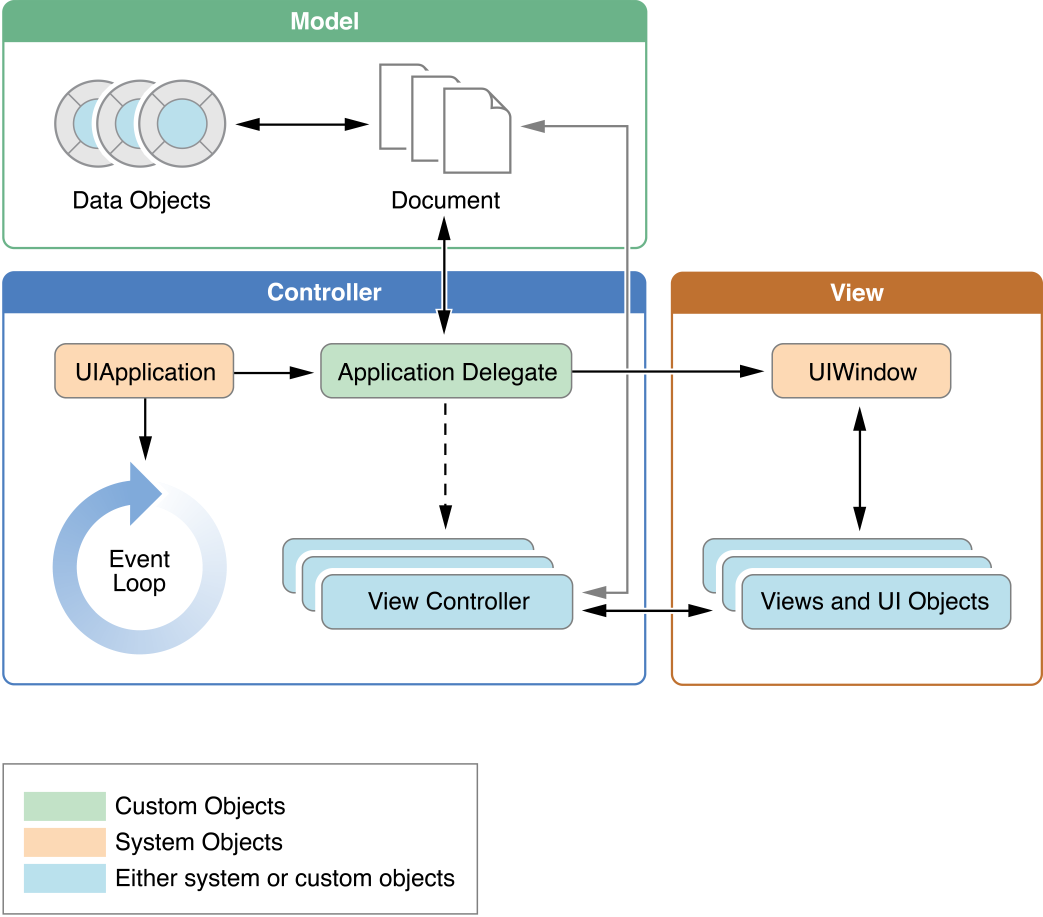
\includegraphics[width=0.9\textwidth]{img/ios_core.png}\\
Application Life Cycle \\

\subsection{Design}
Now I will go over the typical structure of one a TableView Screen in our application with an example from the code. The C7Fit Application consists mainly of these TableView screens, but the principles talked about can be extrapolated to other views like UIView and CollectionViews.\\

\subsubsection{TableViewController}

Taking a look at the HealthKitTableViewController.swift we can see the general structure of the defined class: \\

\begin{lstlisting}[language=Swift]
class HealthKitTableViewController: UITableViewController {
    
    // MARK: - Properties
    let healthInfoID = "healthInfo"
    var healthKitManager = HealthKitManager()
    
    // MARK: - View Life cycle
    override func viewDidLoad() {
    	...
        healthKitManager.authorizeHealthKit()
        self.title = "Today's Activity"
    	...
    }
    override init(style: UITableViewStyle) {
    	...
    }
    required init?(coder aDecoder: NSCoder) {
    	...
    }
    // MARK: - Table view delegate
    override func numberOfSections(in tableView: UITableView) -> Int {
        return 2
    }
    override func tableView(_ tableView: UITableView, numberOfRowsInSection section: Int) -> Int {
        switch section {
        case 0:
            return 4
        case 1:
            return 2
        default:
            return 0
        }
    }
    override func tableView(_ tableView: UITableView, titleForHeaderInSection section: Int) -> String? {
        switch section {
        case 0:
            return "Health Statistics"
        case 1:
            return "Recent Activity"
        default:
            return "Other Statistics"
        }
    }
    // MARK: - Table view data source
    
        override func tableView(_ tableView: UITableView, cellForRowAt indexPath: IndexPath) -> UITableViewCell {
        switch indexPath.section {
        case 0:
            switch indexPath.row {
            case 0:
                let sampleType = HKSampleType.quantityType(forIdentifier: HKQuantityTypeIdentifier.bodyMass)
                let titleLabel = "Weight"
                return queryData(titleLabel: titleLabel, sampleType: sampleType!, path: indexPath)
            case 1:
                ...
            case 2:
                ...
            ...
            default:
                break
            }
		case 1:
        	...

        return UITableViewCell()
    }
    ... Function of the class ...
}
\end{lstlisting}
Starting from the beginning of the class definition, on line one, we can see that the TableViewController inherits the UITableViewController delegate. This means that within our new class we have to explicitly define a set of protocols that outlined by the delegate. \\

The first section of the class is the defined as the properties of the class. These are variables defined that need to be used within the global scope of the class. Most commonly they will be instances of data managers, title strings, cell reuse IDs, etc.\\

Following the properties, we have functions of the View Life Cycle. These functions are required and are called when the view is instantiated. Within these functions, there are a few required function calls initiated when Swift creates the skeleton function, and here we set up anything that must be loaded and defined once the view has been set up like permissions and titles. \\

Next is the delegate which outlines the look of the TableView. Here in the HealthKitTableView it defines the number of sections, rows, and titles for each row. There are other delegate protocols from UITableViewController that can define row height, section type, editing, button types, etc. \\

The last delegate methods are the data source methods. These methods define the function of the TableView, hence their name data source. This is where the contents of the cell and it is pulled from the ViewCell.

\subsubsection{ViewCell}
TableViewControllers make use of ViewCells to populate their cells. Keeping these separate from the Controller class allows reuse of common cells for added simplicity and efficiency. We will continue with the previous example and show the structure of the HealthInfoCell a simple TableViewCell.

\begin{lstlisting}[language=Swift]
class HealthInfoCell: UITableViewCell {

    // MARK: - Properties
    var titleLabel = UILabel()
    var infoLabel = UILabel()

    // MARK: - Initialization
    override init(style: UITableViewCellStyle, reuseIdentifier: String?) {
        super.init(style: style, reuseIdentifier: reuseIdentifier)
        setup()
        setupConstraints()
    }

    required init?(coder aDecoder: NSCoder) {
    	...
    }

    // MARK: - Layout
    func setup() {
        addSubview(titleLabel)
        addSubview(infoLabel)
    }

    func setupConstraints() {
        titleLabel.translatesAutoresizingMaskIntoConstraints = false
        let titleLead = titleLabel.leadingAnchor.constraint(equalTo: leadingAnchor, constant: 10)
        let titleTop = titleLabel.topAnchor.constraint(equalTo: topAnchor, constant: 10)
        let titleBottom = titleLabel.bottomAnchor.constraint(equalTo: bottomAnchor, constant: -10)
        NSLayoutConstraint.activate([titleLead, titleTop, titleBottom])

        infoLabel.translatesAutoresizingMaskIntoConstraints = false
  		...
        NSLayoutConstraint.activate([infoTrail, infoTop, infoBottom])
    }

}
\end{lstlisting}

From this example we can see that the structure begins similar to the TableViewController where common properties are defined at the top of the class. Continuing with that trend, right below the initialization functions initialize the cell by calling two setup functions that are defined below. These initialization functions have some functions that need to be defined in order for the delegate requirement to be satisfied.\\

Looking at the layout of the cell we can see that both the UILabels from the property section are added to our ViewCell. There is no text within them because if we go back to the TableViewController we can see that we defined the titles. This flexibility lets us use this one ViewCell structure for a multitude of cells in the TableView.\\

Finally, the last function sets up the constraints of the view. For our application, we coded all of our views using constraints, which means that we did not use any of Apple's drag and drop tools like Interface Builder. To do this we define some constraints on each of the UILabels to determine their appearance: the titleLabel in this case is constrained 10 units to the right of the left of the cell (leading), and 10 units above and below the bottom and top of the cell respectively. Anchors are the iOS defined hard properties of each view item, and in this case the dimensions of the cell defined within the overall TableViewController.\\

\subsection{Firebase}

The Firebase data manager is an essential part of our application as it handles all of the application's communications with the offline Firebase server. Fortunately, most of the hard work with Firebase is already done by Google and our manager. To use Firebase within our application all that needs to be done is to import Firebase, initialize the manager, and authenticate the user.\\

\begin{lstlisting}[language=Swift]
import Firebase
let firebaseDataManager = FirebaseDataManager()
firebaseDataManager.monitorLoginState { _, user in
	guard let userID = user?.uid else { return self.present(LoginViewController(), animated: true, completion: nil) }
    \\ Execute Code Here        
}
\end{lstlisting}

The above code shows an example of how to use Firebase within our application. The data manager's monitorLoginState will handle user login if the user is not already authenticated, so all that needs to be done is encapsulate any Firebase related code within this wrapper function. More documentation on the usage of Firebase can be found on the Google Documentation site at https://firebase.google.com/docs/ios/setup. \\

\subsection{Ebay API}
Our application uses the eBay API to query for information on various gym related items. To do this we need to access the eBay API which uses oAuth for authentication. There was a discrepancy with their oAuth as it didn't conform to the standard oAuth protocols so our application has a wrapper function within the EbayAPITokenManager to handle this. One problem is that the oAuth token will expire after a certain amount of time, and so the application needs to be restarted after a certain amount of time or eBay queries will not respond. The ebayDataManager has two functions that allow easy searching and getting items. Below is a code snippet that shows a query in action. \\ 

\begin{lstlisting}[language=Swift]
let ebayAPITokenManager = EbayAPITokenManager()
let ebayDataManager = EbayDataManager()

ebayAPITokenManager.getOAuth2Token { OAuth2Token in
        guard let token = OAuth2Token else { return }
        self.ebayAPIToken = OAuth2Token
        self.ebayDataManager.searchItem(query: "Yoga Ball", OAuth2Token: token) { itemCategory in
           guard let itemCategory = itemCategory else { return }
           self.categoryCellData.append(itemCategory)
           self.collectionView?.reloadData()
       }
       self.ebayDataManager.searchItem(query: "Gym Shoes", OAuth2Token: token) { itemCategory in
       		...
       }
       ...
}
\end{lstlisting}
